\documentclass{scrartcl}

\usepackage{ucs}
\usepackage[utf8x]{inputenc}
\usepackage[english]{babel}
\usepackage{graphicx}
\usepackage{amsmath}
\usepackage{amssymb}
\usepackage{mathtools}
\usepackage{titlesec}
\usepackage[table]{xcolor}
\usepackage{listings}
\usepackage{tikz}
\usepackage{pgfplots}
\usepackage{environ}
\usepackage{subcaption}
\usepackage{svg}

\captionsetup[subfigure]{
	list=true, 
	font=large, 
	labelfont=bf, 
	labelformat=brace, 
	position=top
}

\DeclarePairedDelimiter\abs{\lvert}{\rvert}%
\DeclarePairedDelimiter\norm{\lVert}{\rVert}%

% Swap the definition of \abs* and \norm*, so that \abs
% and \norm resizes the size of the brackets, and the 
% starred version does not.
\makeatletter
\let\oldabs\abs
\def\abs{\@ifstar{\oldabs}{\oldabs*}}
%
\let\oldnorm\norm
\def\norm{\@ifstar{\oldnorm}{\oldnorm*}}
\makeatother

\newcommand*{\Value}{\frac{1}{2}x^2}%

\usetikzlibrary{matrix,chains,positioning,decorations.pathreplacing,arrows,calc}

\makeatletter
\newsavebox{\measure@tikzpicture}
\NewEnviron{scaletikzpicturetowidth}[1]{%
	\def\tikz@width{#1}%
	\def\tikzscale{1}\begin{lrbox}{\measure@tikzpicture}%
		\BODY
	\end{lrbox}%
	\pgfmathparse{#1/\wd\measure@tikzpicture}%
	\edef\tikzscale{\pgfmathresult}%
	\BODY
}
\makeatother

\lstset{
	language=Python,
	frame=tb,
	commentstyle=\color{darkgray},
	breaklines=true
}

\tikzset{
	block/.style={
		draw,
		rectangle, 
		text width=3em, 
		text centered, 
		minimum height=8mm,     
		node distance=2.3em
	}, 
	line/.style={draw}
}

\setcounter{secnumdepth}{4}

\titleformat{\paragraph}
{\normalfont\normalsize\bfseries}{\theparagraph}{1em}{}
\titlespacing*{\paragraph}
{0pt}{3.25ex plus 1ex minus .2ex}{1.5ex plus .2ex}

\setlength\parindent{0pt}

\title{Inhaltbasierte Bild- und Videoanalyse \\ Zusammenfassung}
\author{Thomas Mohr}
\date{}

\begin{document}
\maketitle
\pagebreak
\tableofcontents
\pagebreak

\section{Introduction}

\subsection{Data vs. Information Retrieval}

\begin{tabular}{|c|c|c|}
	\hline 
	Aspect & Data Retrieval & Information Retrieval \\ 
	\hline \hline
	Information & explicit & implicit \\ 
	\hline 
	Model & deterministic & probabilistic \\ 
	\hline 
	Results & exact & fuzzy \\ 
	\hline 
	Query & once & iterative refinement \\ 
	\hline 
	Fault tolerance & none & yes \\ 
	\hline 
	Result collection & set & list \\ 
	\hline 
\end{tabular} 

\subsection{Different Color Spaces}

\begin{itemize}
	\item RGB: Red, Green, Blue
	\begin{itemize}
		\item Monitor and display technology
		\item Easily usable from a programmer's perspective
		\item RGB is non-linear
		\item If RGB value changes: Hue \textbf{and} saturation \textbf{and} brightness change
		\item Appearance of colors depends on output device
	\end{itemize}	\begin{tabular}{|c|l||c|c|c|}
		\hline 
		Abbr. & Color & R & G & B \\ 
		\hline 
		\textbf{S} & Black & 0.00 & 0.00 & 0.00 \\ 
		\textbf{R} & Red & 1.00 & 0.00 & 0.00 \\ 
		\textbf{Y} & Yellow & 1.00 & 1.00 & 0.00 \\ 
		\textbf{G} & Green & 0.00 & 1.00 & 0.00 \\ 
		\textbf{C} & Cyan & 0.00 & 1.00 & 1.00 \\ 
		\textbf{B} & Blue & 0.00 & 0.00 & 1.00 \\ 
		\textbf{M} & Magenta & 1.00 & 0.00 & 1.00 \\ 
		\textbf{W} & White & 1.00 & 1.00 & 1.00 \\ 
		\hline 
		\textbf{K} & 50\% Gray & 0.50 & 0.50 & 0.50 \\ 
		\hline 
		$ \mathbf{R}_{75} $ & 75\% Red & 0.75 & 0.00 & 0.00 \\ 
		$ \mathbf{R}_{50} $ & 50\% Red & 0.50 & 0.00 & 0.00 \\ 
		$ \mathbf{R}_{25} $ & 25\% Red & 0.25 & 0.00 & 0.00 \\ 
		\hline 
		\textbf{P} & Pink & 1.00 & 0.50 & 0.50 \\ 
		\hline 
	\end{tabular} 
	\item $ YC_bC_r $
	\begin{itemize}
		\item $ Y $: Luminance
		\item $ C_b $: Blue difference level
		\item $ C_r $: Red difference level
	\end{itemize}
	\item HSB/HSV/HLS
	\begin{itemize}
		\item Hue
		\item Saturation
		\item Brightness (or Value, or Lightness)
	\end{itemize}
\end{itemize}

\subsubsection{Color Space Conversion (RGB2HSV)}

\begin{align*}
	V &\leftarrow max(R,G,B) \\
	S &\leftarrow \begin{cases}
		\frac{V-min(R,G,B)}{V} & \text{if } V \neq 0 \\
		0 & \text{otherwise}
	\end{cases} \\
	H & \leftarrow \begin{cases}
		\frac{60(G-B)}{V-min(R,G,B)} & \text{if } V=R \\
		\frac{120+60(B-R)}{V-min(R,G,B)} & \text{if } V=G \\
		\frac{240+60(R-G)}{V-min(R,G,B)} & \text{if } V=B
	\end{cases}
\end{align*}

\subsubsection{Color Spaces for TV (Television)}

\begin{itemize}
	\item YUV/$ YC_bC_r $: Color space(s) for standardized recording, storage, transmission and display of color TV video (frames)
	\item Color space is seperated in (analog TV)
	\begin{itemize}
		\item 1 luminance component $ Y $
		\item 2 color components $ U,V $
	\end{itemize}
	\item $ YUV \rightarrow $ PAL/NTSC analog TV
	\item $ YC_bC_r \rightarrow $ digital TV
\end{itemize}

\subsubsection{YUV (Component) Color Space}

\begin{itemize}
	\item Color space conversion: RGB $ \rightarrow $ YUV
	\begin{align*}
		Y &= 0.299*R+0.587*G+0.114*B \\
		U &= 0.492*(B-Y) \\
		V &= 0.877*(R-Y)
	\end{align*}
	\item In matrix form (linear mapping)
	\begin{itemize}
		\item RGB $ \rightarrow $ YUV
		\begin{align*}
			\begin{pmatrix}
				Y \\
				U \\
				V
			\end{pmatrix} = \begin{bmatrix}
				0.299 & 0.587 & 0.114 \\
				-0.147 & -0.289 & 0.436 \\
				0.615 & -0.515 & -0.100
			\end{bmatrix} * \begin{pmatrix}
				R \\
				G \\
				B
			\end{pmatrix}
		\end{align*}
		\item YUV $ \rightarrow $ RGB
		\begin{align*}
			\begin{pmatrix}
				R \\
				G \\
				B
			\end{pmatrix} = \begin{bmatrix}
				1.000 & 0.000 & 1.140 \\
				1.000 & -0.395 & -0.581 \\
				1.000 & 2.032 & 0.000
			\end{bmatrix} * \begin{pmatrix}
				Y \\
				U \\
				V
			\end{pmatrix}
		\end{align*}
	\end{itemize}
\end{itemize}

\subsubsection{$ YC_bC_r $ Component Color Space}

\begin{itemize}
	\item Variant (extension) of YUV
	\item International standard for digital TV
	\item Common for JPEG (JFIF, EXIF)
	\item RGB $ \rightarrow YC_bC_r $
	\begin{align*}
		\begin{pmatrix}
			Y \\
			C_b \\
			C_r
		\end{pmatrix} = \begin{bmatrix}
			0.299 & 0.587 & 0.114 \\
			-0.169 & -0.331 & 0.500 \\
			0.500 & -0.419 & -0.081
		\end{bmatrix} * \begin{pmatrix}
			R \\
			G \\
			B
		\end{pmatrix}
	\end{align*}
	\item $ YC_bC_r \rightarrow $ RGB
	\begin{align*}
		\begin{pmatrix}
			R \\
			G \\
			B
		\end{pmatrix} = \begin{bmatrix}
			1.000 & 0.000 & 1.403 \\
			1.000 & -0.334 & -0.714 \\
			1.000 & 1.173 & 0.000
		\end{bmatrix} * \begin{pmatrix}
			Y \\
			C_b \\
			C_r
		\end{pmatrix}
	\end{align*}
\end{itemize}

\subsection{Evaluation of Multimedia Retrieval Systems}

\begin{itemize}
	\item Speed of answering queries
	\item Judge relevance of retrieved document
	\item Popular measures
	\begin{itemize}
		\item Recall
		\item Precision
		\item Average precision
	\end{itemize}
\end{itemize}

\subsubsection{Performance Measures}

\begin{itemize}
	\item Recall \\
	''Probability'' that a relevant document is found (recognition rate)
	\item Precision \\
	''Probability'' that a found document is relevant
	\item Average precision \\
	Averaged precision across all ranks with a relevant document for a result list
\end{itemize}

\paragraph{Recall \& Precision}

\begin{itemize}
	\item Given are
	\begin{itemize}
		\item R \\
		Number of relevant objects or events in test data set
		\item C \\
		Number of correctly detected relevant objetcs/events
		\item D \\
		Number of detected objects/events, including the irrelevant ones (''false alarms'')
	\end{itemize}
	\item Therefore
	\begin{align*}
		\text{recall} &= \frac{C}{R} \\
		&= \frac{\text{true positives}}{\text{true positives}+\text{false positives}} \\
		\text{precision} &= \frac{C}{D} \\
		&= \frac{\text{true positives}}{\text{true positives}+\text{false negatives}}
	\end{align*}
	\item F1 measure is a combination of both, harmonic mean
	\begin{align*}
		f1=\frac{2*\text{recall}*\text{precision}}{\text{recall}+\text{precision}}
	\end{align*}
\end{itemize}

\begin{figure}[ht!]
	\centering
	\includegraphics[width=0.7\linewidth]{figures/Precisionrecall.pdf}
	\caption{Precision/Recall}
	\label{fig:precision_recall}
\end{figure}


\paragraph{Average Precision}

\begin{itemize}
	\item $ A $ is the result set of returned documents
	\item $ L_k=\{I_1,\ldots,I_k\} $ is the subset of the $ k $ most similiar responses
	\item $ R $ ist the set of returned relevant documents in the top-k response
	\item $ R_{all} $ is the set of all relevant documents in the entire data collection
	\item $ \psi(I_i) $ is a function that is
	\begin{itemize}
		\item 1 if $ I_i \in R $
		\item 0 if $ I_i \not \in R $
	\end{itemize}
\end{itemize}

\begin{align*}
	avg\_precision &= \frac{1}{\abs{R_{all}}} \sum_{k=1}^{\abs{A}} \frac{\abs{R \cap L^k}}{k} \psi(l_k) \\
	avg\_precision &*= \frac{1}{\abs{R_{result\_set}}} \sum_{k=1}^{\abs{A}} \frac{\abs{R \cap L^k}}{k} \psi(l_k)
\end{align*}

\begin{enumerate}
	\item \textbf{relevant document} (precision@1:100\%)
	\item irrelevant document
	\item irrelevant document
	\item \textbf{relevant document} (precision@4:50\%)
	\item irrelevant document
	\item \textbf{relevant document} (precision@6:50\%)
	\item irrelevant document
	\item irrelevant document
\end{enumerate}

\begin{align*}
	\text{average precision} &: \frac{200}{3}=67\% \\
	\text{precision overall} &: 37,5\%
\end{align*}

\subsubsection{Recall-Precision Curve}

\begin{figure}[ht!]
	\centering
	\includegraphics[width=0.7\linewidth]{figures/precision_recall.png}
	\caption{Average precision approximates the area under the curve}
	\label{fig:precision_recall_curve}
\end{figure}


\pagebreak
\section{Image Classification}

\subsection{Challenges}

\begin{itemize}
	\item Semantic Gap
	\begin{itemize}
		\item An image is just a big grid of numbers between [0,255]
	\end{itemize}
	\item Viewpoint Variation
	\begin{itemize}
		\item All pixels change when the camera moves
	\end{itemize}
	\item Illumination (Lighting)
	\item Deformation (Shape)
	\item Occlusion
	\item Background Clutter (Similiar background pattern)
	\item Intraclass Variation
\end{itemize}

\subsection{Machine Learning Algorithms}

\begin{itemize}
	\item Supervised Learning (''right answers'' given)
	\begin{itemize}
		\item Classification \\
		discrete valued output
		\item Regression \\
		continuous valued output
	\end{itemize}
	\item Unsupervised Learning
	\begin{itemize}
		\item Find hidden structure from unlabeled data
		\item No ground truth given
		\item Clustering
		\item Dimensionality reduction
	\end{itemize}
\end{itemize}

\subsubsection{Nearest Neighbor}

\begin{itemize}
	\item Nearest Neighbor
	\begin{itemize}
		\item Memorize all data and labels
		\item Predict the label of most similiar training image
	\end{itemize}
	\item K-Nearest Neighbor
	\begin{itemize}
		\item Instead of copying label from nearest neighbor, take \textbf{majority vote} from $ K $ closest points
		\item Never used on images
		\begin{itemize}
			\item Very slow at test time
			\item Distance metrics on pixels are not informative. The following share the same L2 distance:
			\begin{itemize}
				\item Original
				\item Boxed
				\item Shifted
				\item Tinted
			\end{itemize}
		\end{itemize}
	\end{itemize}
\end{itemize}

\subsubsection{Distance metrics}

\begin{itemize}
	\item L1 (Manhattan) distance
	\begin{align*}
		d_1(I_1,I_2)=\sum_{p} \abs{I_1^p-I_2^p}
	\end{align*}
	\begin{align*}
		\abs{
			\overset{\text{test image}}{\begin{tabular}{|c|c|c|c|}
				\hline 
				56 & 32 & 10 & 18 \\ 
				\hline 
				90 & 23 & 128 & 133 \\ 
				\hline 
				24 & 26 & 178 & 200 \\ 
				\hline 
				2 & 0 & 255 & 220 \\ 
				\hline 
				\end{tabular} }
			-
			\overset{\text{training image}}{\begin{tabular}{|c|c|c|c|}
				\hline 
				10 & 20 & 24 & 17 \\ 
				\hline 
				8 & 10 & 89 & 100 \\ 
				\hline 
				12 & 16 & 178 & 170 \\ 
				\hline 
				4 & 32 & 233 & 112 \\ 
				\hline 
				\end{tabular} }
		}
		=
		\overset{\text{pixel-wise absolute value differences}}{\begin{tabular}{|c|c|c|c|}
			\hline 
			46 & 12 & 14 & 1 \\ 
			\hline 
			82 & 13 & 39 & 33 \\ 
			\hline 
			12 & 10 & 0 & 30 \\ 
			\hline 
			2 & 32 & 22 & 108 \\ 
			\hline 
			\end{tabular} }
		\overset{\text{add}}{\rightarrow} 456
	\end{align*}
	\item L2 (Euclidean) distance
	\begin{align*}
		d_2(I_1,I_2)=\sqrt{\sum_{p} (I_1^p-I_2^p)^2}
	\end{align*}
\end{itemize}

\subsubsection{Hyperparameters}

\begin{itemize}
	\item What is the best value of $ \mathbf{k} $ to use?
	\begin{itemize}
		\item Split data into train, validation and test
		\item Cross-Validation
		\begin{itemize}
			\item Split data into \textbf{folds}, try each fold as validation and average the results
			\item Useful for small datasets, but not used too frequently in deep learning
		\end{itemize}
	\end{itemize}
	\item What is the best \textbf{distance} to use?
	\begin{itemize}
		\item L1 distance
		\item L2 distance
	\end{itemize}
	\item These are \textbf{hyperparameters}: Choices about the algorithm that we set rather than learn
\end{itemize}

\subsection{Linear Classification}

\begin{itemize}
	\item Score function
	\begin{align*}
		f(x,W)=Wx+b
	\end{align*}
	\begin{itemize}
		\item Input: Image of a cat with 4 pixels
		\item Output: Score for each class
	\end{itemize}
	\begin{align*}
		\overset{\text{input image} (x)}{
			\begin{tabular}{|c|c|}
				\hline 
				56 & 231 \\ 
				\hline 
				24 & 2 \\ 
				\hline 
			\end{tabular}
		}
	\end{align*}
	\begin{align*}
		\overset{W}{
			\begin{tabular}{|c|c|c|c|}
				\hline 
				0,2 & -0,5 & 0,1 & 2,0 \\ 
				\hline 
				1,5 & 1,3 & 2,1 & 0,0 \\ 
				\hline 
				0 & 0,25 & 0,2 & -0,3 \\ 
				\hline 
			\end{tabular}
		}
		\times
		\overset{x}{
			\begin{tabular}{|c|}
				\hline 
				56 \\ 
				\hline 
				231 \\ 
				\hline 
				21 \\ 
				\hline 
				2 \\ 
				\hline 
			\end{tabular}
		}
		+
		\overset{b}{
			\begin{tabular}{|c|}
				\hline 
				1,1 \\ 
				\hline 
				3,2 \\ 
				\hline 
				-1,2 \\ 
				\hline 
			\end{tabular}
		}
		=
		\begin{tabular}{|c|}
			\hline 
			-96,8 \\ 
			\hline 
			437,9 \\ 
			\hline 
			61,95 \\ 
			\hline 
		\end{tabular} 
		\begin{tabular}{c}
			\textbf{cat} \\ 
			dog \\ 
			ship \\ 
		\end{tabular} 
	\end{align*}
	\item Loss function
	\begin{align*}
		\frac{1}{N} \sum_i L_i(f(x_i,W),y_i)
	\end{align*}
	\begin{itemize}
		\item Tells how good the current classifier ist
		\item Given a dataset of examples $ \{ (x_i,y_i) \}_{i=1}^N $
		\begin{itemize}
			\item $ x_i $ is an image
			\item $ y_i $ is an (integer) label
		\end{itemize}
	\end{itemize}
	\item Multiclass SVM Loss
	\begin{itemize}
		\item ''Hinge loss''
		\begin{align*}
			L_i &= \sum_{j \not = y_i} \begin{cases}
				0 & \text{if } s_{y_i} \leq s_j+1 \\
				s_j-s_{y_i}+1 & \text{otherwise}
			\end{cases} \\
			&= \sum_{j \not = y_i} \max (0,s_j-s_{y_i}+1)
		\end{align*}
	\end{itemize}
\end{itemize}

\subsection{Regularization}

\begin{align*}
	L(W)=
	\underbrace{\frac{1}{N} \sum_{i=1}^{N} L_i(f(x_i,W),y_i)}_{\substack{\text{\textbf{Data loss:} Model predictions} \\ \text{should match training data}}}
	+
	\underbrace{\lambda R(W)}_{\substack{\text{\textbf{Regularization}: Model} \\ \text{should be ''simple'', so it} \\ \text{works on test data}}}
\end{align*}

\begin{itemize}
	\item \textbf{L2 regularization} \hfill $ R(W) = \sum_k \sum_l W_{k,l}^2 $
	\item L1 regularization \hfill $ R(W) = \sum_k \sum_l \abs{W_{k,l}} $
	\item Elastic net (L1+L2) \hfill $ R(W) = \sum_k \sum_l \beta W_{k,l}^2 + \abs{W_{k,l}} $
	\item Max norm regularization
	\item Dropout
	\item Batch normalization
\end{itemize}

\pagebreak
\section{Neural Networks Intro}

\subsection{Softmax Classifier}

\begin{itemize}
	\item \textbf{Given}: score function
	\begin{align*}
		s=f(x_i,W)
	\end{align*}
	\item \textbf{Wanted}: probability distribution over $ K $ different possible outcomes
	\item \textbf{Softmax function} ''squashes'' a $ K $-dimensional vector of
	 arbitrary real values to a $ K $-dimensional vector of real values in the range [0,1] that add up to 1
	\begin{align*}
		P(Y=k \mid X=x_i)=\Aboxed{\frac{e^s_{k}}{\sum_j e^s_{j}}}
	\end{align*}
\end{itemize}

\subsubsection{Loss function for Softmax Classifier}

Want to maximize the log likelihood \\
$ \rightarrow $ minimize the negative log likelihood of the correct class:

\begin{figure}[ht]
	\begin{minipage}[b]{0.45\linewidth}
		\centering
		\begin{align*}
			L_i&=-\log P(Y=y_i \mid X=x_i) \\
			&=-\log (\frac{e^{s_{y_i}}}{\sum_j e^{s_j}})
		\end{align*}
		\caption{Log loss formula}
		\label{fig:figure1}
	\end{minipage}
	\hspace{0.5cm}
	\begin{minipage}[b]{0.45\linewidth}
		\centering
		\includegraphics[width=\textwidth]{figures/Log_loss_graph.png}
		\caption{Log loss plot}
		\label{fig:figure2}
	\end{minipage}
\end{figure}

\subsubsection{Softmax Classifier Example}

\begin{align*}
	\begin{tabular}{l}
		cat \\ 
		car \\ 
		frog \\ 
	\end{tabular} 
	\begin{tabular}{|c|}
		\arrayrulecolor{blue}
		\hline
		\textbf{3.2} \\ 
		5.1 \\ 
		-1.7 \\ 
		\hline
	\end{tabular}
	\begin{tabular}{c}
		\\ 
		$ \overset{\exp}{\rightarrow} $ \\ 
		\\ 
	\end{tabular} 
	\begin{tabular}{|c|}
		\arrayrulecolor{red}
		\hline
		\textbf{24.5} \\ 
		164.0 \\ 
		0.18 \\ 
		\hline
	\end{tabular}
	\begin{tabular}{c}
		\\ 
		$ \overset{\text{normalize}}{\rightarrow} $ \\ 
		\\ 
	\end{tabular} 
	\begin{tabular}{|c|}
		\arrayrulecolor{green}
		\hline
		\textbf{0.13} \\ 
		0.87 \\ 
		0.00 \\ 
		\hline
	\end{tabular}
	\begin{tabular}{c}
		$ \rightarrow L_i=-\log (0.13)=0.89 $ \\ 
		\\ 
		\\ 
	\end{tabular} \\
	\textcolor{blue}{\text{unnormalized log probabilities}}
	\rightarrow
	\textcolor{red}{\text{unnormalized probabilities}}
	\rightarrow
	\textcolor{green}{\text{probabilities}}
\end{align*}

\subsection{Gradients}

\subsubsection{Following the gradient}

\begin{itemize}
	\item In 1-dimension, the derivative of a function:
	\begin{align*}
		\frac{df(x)}{dx}=\lim\limits_{h\rightarrow0}\frac{f(x+h)-f(x)}{h}
	\end{align*}
	\item In multiple dimensions, the \textbf{fradient} is the vector of (partial derivatives) along each dimension
	\item The slope in any direction is the \textbf{dot product} of the direction with the gradient
	\item The direction of the steepest descent is the \textbf{negative gradient}
\end{itemize}

\subsubsection{Computing the gradient}

\begin{itemize}
	\item \textbf{Numerical} gradient
	\begin{itemize}
		\item Easy way
		\item Slow
		\item Approximate
	\end{itemize}
	\item \textbf{Analytic} gradient
	\begin{itemize}
		\item Fast
		\item Exact
		\item More error-prone
	\end{itemize}
\end{itemize}

\subsubsection{Gradient descent}

\begin{itemize}
	\item Procedure of repeatedly evaluating the gradient and then performing a parameter update
	\item Variants
	\begin{itemize}
		\item Vanilla/Batch gradient descent
		\begin{lstlisting}
while True:
	weights_grad = evaluate_gradient(
		loss_fun, 
		data, 
		weights
	)
	# perform parameter update
	weights += -step_size * weights_grad
		\end{lstlisting}
		\item Mini-batch gradient descent
		\begin{lstlisting}
while True:
	# sample 256 examples
	data_batch = sample_training_data(data, 256)
	weights_grad = evaluate_gradient(
		loss_fun, 
		data_batch, 
		weights
	)
	# perform parameter update
	weights += -step_size * weights_grad
		\end{lstlisting}
		\item Stochastic gradient descent
		\begin{itemize}
			\item Mini-batch with only a single example (at a time)
		\end{itemize}
	\end{itemize}	
	\item Follow the gradient until we're happy with the results
	\item Core of all Neural Network libraries
\end{itemize}

\paragraph{Effect of step size}

\begin{itemize}
	\item The gradient only tells us the direction
	\item How far should we step along this direction?
	\item \textbf{Step size (learning rate)}: \\
	Most important hyperparameter setting in training neural networks
	\begin{itemize}
		\item Small step size $ \rightarrow $ make consistent, but very small progress
		\item Large step size $ \rightarrow $ attempt to descend faster, may fail
	\end{itemize}
\end{itemize}

\begin{figure}[ht!]
	\centering
	\begin{minipage}[b]{0.4\textwidth}
		\includegraphics[width=\textwidth]{figures/sgd_small_step_size.png}
		\caption{Small step size}
	\end{minipage}
	\hfill
	\begin{minipage}[b]{0.4\textwidth}
		\includegraphics[width=\textwidth]{figures/sgd_large_step_size.png}
		\caption{Large step size}
	\end{minipage}
\end{figure}

\subsection{Backpropagation}

\begin{itemize}
	\item Resursive application of the chain rule along a computational graph to compute the gradients of all inputs/parameters/intermediates
	\item Calculate the gradient of the loss function with respect to the weights/inputs
	\item Phases
	\begin{itemize}
		\item Propagation
		\begin{itemize}
			\item Forward propagation of a training pattern's input through the neural network in order to generate the network's output value(s).
			\item Backward propagation of the propagation's output activations through the neural network using the training pattern target in order to generate the deltas (the difference between the targeted and actual output values) of all output and hidden neurons.
		\end{itemize}
		\item Weight update
		\begin{itemize}
			\item For each weight the following steps must be followed:
			\begin{itemize}
				\item The weight's output delta and input activation are multiplied to find the gradient of the weight.
				\item A ratio (percentage) of the weight's gradient is subtracted from the weight.
			\end{itemize}
			\item This ratio (percentage) influences the speed and quality of learning; it is called the learning rate. The greater the ratio, the faster the neuron trains, but the lower the ratio, the more accurate the training is. The sign of the gradient of a weight indicates whether the error varies directly with, or inversevely to, the weight. Therefore, the weight must be updated in the opposite direction, ''descending'' the gradient.
		\end{itemize}
	\end{itemize}
\end{itemize}

\begin{figure}[ht!]
	\caption{Backpropagation}
	\centering
	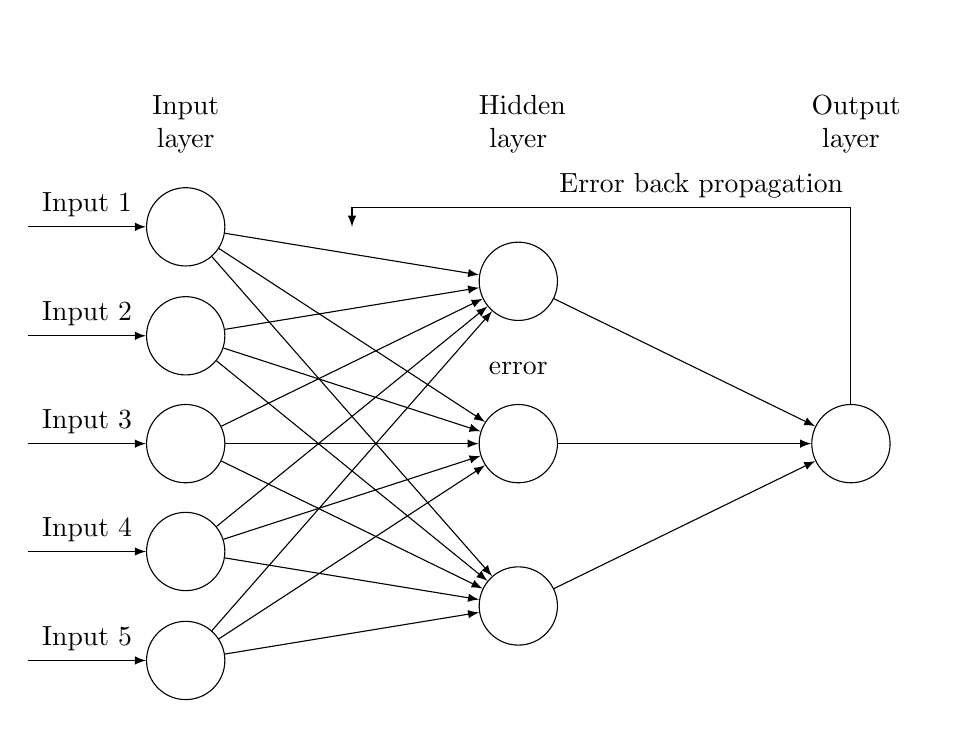
\begin{tikzpicture}[
	plain/.style={
		draw=none,
		fill=none,
	},
	net/.style={
		matrix of nodes,
		nodes={
			draw,
			circle,
			inner sep=10pt
		},
		nodes in empty cells,
		column sep=2cm,
		row sep=-9pt
	}, 
	>=latex
	]
	\matrix[net] (mat)
	{ 
		|[plain]| \parbox{1cm}{\centering Input\\layer} & |[plain]| \parbox{1cm}{\centering     Hidden\\layer} & |[plain]| \parbox{1cm}{\centering Output\\layer} \\
		& |[plain]| \\
		|[plain]| & \\
		& |[plain]| \\
		|[plain]| & |[plain]| \\
		& & \\
		|[plain]| & |[plain]| \\
		& |[plain]| \\
		|[plain]| & \\
		& |[plain]| \\
	};
	\foreach \ai [count=\mi ]in {2,4,...,10}
	\draw[<-] (mat-\ai-1) -- node[above] {Input \mi} +(-2cm,0);
	\foreach \ai in {2,4,...,10}
	{\foreach \aii in {3,6,9}
		\draw[->] (mat-\ai-1) -- (mat-\aii-2);
	}
	\foreach \ai in {3,6,9}
	\draw[->] (mat-\ai-2) -- (mat-6-3);
	%\draw[->] (mat-6-3) -- node[above] {Ouput} +(2cm,0);
	\path [line] node{error} -- (mat-1-1);
	\draw[->] (mat-6-3) -- ++(0pt,3cm) -| node[pos=0.15,above] {Error back propagation} ( $ (mat-2-1)!0.5!(mat-2-2) $ );
	\end{tikzpicture}
\end{figure}

\subsubsection{Gates}

\begin{itemize}
	\item Add \\ Gradient distributor (both operands gradients are set to backpropagated gradient)
	\item Max \\ Gradient router (maximum input of operands receives gradient; other operand is set to 0.00)
	\item Mul \\ Gradient switcher (gradient multiplied by input from other operand)
\end{itemize}

\subsubsection{Vectorized operations}

\begin{itemize}
	\item Jacobi matrix \\ TODO
\end{itemize}

\subsection{Neurons}

\begin{figure}[ht!]
	\caption{Neuron}
	\centering
	\includegraphics[width=\textwidth]{figures/neuron_model.jpeg}
\end{figure}

\subsection{Activation functions}

\begin{figure}[ht!]
	\begin{subfigure}[c]{0.5\textwidth}
		\begin{scaletikzpicturetowidth}{\textwidth}
			\begin{tikzpicture}[scale=\tikzscale]
				\begin{axis}
					[
						domain=-10:10,
						samples=150,
						scale only axis,
						axis y line=middle, 
						axis x line=bottom,
						x label style={at={(axis description cs:0.5,-0.1)},anchor=north},
						y label style={at={(axis description cs:-0.1,.5)},rotate=90,anchor=south},
						ymin=0,
						ymax=1,
						ytick={0, 1},
						xmin=-10,
						xmax=10,
						xtick={-10,0,10},
						xlabel={$ x $},
						ylabel=$ \sigma(x) $,
					] 
					\addplot {1/(1+exp(-x))}; 
				\end{axis}
			\end{tikzpicture}
		\end{scaletikzpicturetowidth}
		\subcaption{Sigmoid: $ \sigma(x)=\frac{1}{1+ \exp^{-x}} $}
	\end{subfigure}
	\begin{subfigure}[c]{0.5\textwidth}
		\begin{scaletikzpicturetowidth}{\textwidth}
			\begin{tikzpicture}[scale=\tikzscale]
				\begin{axis}
					[
						domain=-10:10,
						samples=150,
						scale only axis,
						axis y line=middle, 
						axis x line=middle,
						x label style={at={(axis description cs:0.5,-0.1)},anchor=north},
						y label style={at={(axis description cs:-0.1,.5)},rotate=90,anchor=south},
						ymin=-1,
						ymax=1,
						ytick={0, 1},
						xmin=-10,
						xmax=10,
						xtick={-10,0,10},
						xlabel={$ x $},
						ylabel={$ tanh(x) $},
					] 
					\addplot {tanh(x)}; 
				\end{axis}
			\end{tikzpicture}
		\end{scaletikzpicturetowidth}
		\subcaption{$ tanh(x) $}
	\end{subfigure}
	\begin{subfigure}[c]{0.5\textwidth}
		\begin{scaletikzpicturetowidth}{\textwidth}
			\begin{tikzpicture}[scale=\tikzscale]
				\begin{axis}
					[
						domain=-10:10,
						samples=150,
						scale only axis,
						axis y line=middle, 
						axis x line=bottom,
						x label style={at={(axis description cs:0.5,-0.1)},anchor=north},
						y label style={at={(axis description cs:-0.1,.5)},rotate=90,anchor=south},
						ymin=0,
						ymax=10,
						ytick={0, 10},
						xmin=-10,
						xmax=10,
						xtick={-10,0,10},
						xlabel={$ x $},
						ylabel={$ max(0,x) $},
					] 
					\addplot {max(0,x)}; 
				\end{axis}
			\end{tikzpicture}
		\end{scaletikzpicturetowidth}
		\subcaption{ReLU: $ max(0,x) $}
	\end{subfigure}
	\begin{subfigure}[c]{0.5\textwidth}
		\begin{scaletikzpicturetowidth}{\textwidth}
			\begin{tikzpicture}[scale=\tikzscale]
				\begin{axis}
					[
						domain=-10:10,
						samples=150,
						scale only axis,
						axis y line=middle, 
						axis x line=middle,
						x label style={at={(axis description cs:0.5,-0.1)},anchor=north},
						y label style={at={(axis description cs:-0.1,.5)},rotate=90,anchor=south},
						ymin=-1,
						ymax=10,
						ytick={0, 10},
						xmin=-10,
						xmax=10,
						xtick={-10,0,10},
						xlabel={$ x $},
						ylabel={$ max(0.1x,x) $},
					] 
					\addplot {max(0.1*x,x)}; 
				\end{axis}
			\end{tikzpicture}
		\end{scaletikzpicturetowidth}
		\subcaption{Leaky ReLU: $ max(0.1x,x) $}
	\end{subfigure}
\end{figure}

\pagebreak
\section{Image Features}

\subsection{Histograms}

\begin{itemize}
	\item Histograms provide simple image statistics:
	\begin{itemize}
		\item Number of pixels, min and max grey level
		\item Average and standard deviation
		\item Indicator for image quality
	\end{itemize}
	\item Spatial information is lost
	\item Different images can have the same (or a similiar) histogram
\end{itemize}

\subsubsection{Histograms of Color Images}

\begin{itemize}
	\item Luminance histogram
	\begin{itemize}
		\item Distribution of grey level intensities
		\item (can be) computed based on color information
	\end{itemize}
	\item Histograms of color components
	\begin{itemize}
		\item Three histograms: Distribution of intensities in each color channel
		\item Alternative: One combined color histogram
	\end{itemize}
\end{itemize}

\subsection{(Color) Moments of Order 1-3}

\begin{itemize}
	\item Mean of (gray level) image (1. order moment)
	\begin{align*}
		m(I)&=\frac{1}{\sum_{k=0}^{255} h_k} \sum_{k=0}^{255} k * h_k \\
		&=\frac{1}{W*H} \sum_{y=0}^{H-1} \sum_{x=0}^{W-1} i(x,y)
	\end{align*}
	\item Variance (2. order moment, mean squared error)
	\begin{align*}
		\sigma^2(I)=\frac{1}{W*H} \sum_{k=0}^{255} (k-m)^2*h_k
	\end{align*}
	\item Skewness (3. order moment, degree of asymmetry)
	\begin{align*}
		s^3(I)=\frac{1}{W*H} \sum_{k=0}^{255} \frac{(k-m)^3*h_k}{\sigma}
	\end{align*}
	\item Where
	\begin{itemize}
		\item $ h_k $ is entry in bin $ k $
		\item $ W $ is the width of the image
		\item $ H $ is the height of the image
	\end{itemize}
\end{itemize}

\subsection{Color Correlogram}

\begin{itemize}
	\item Given a color $ c $, e.g., $ (r,g,b) \rightarrow $ what is the probability that a pixel of color $ c' $ appears in distance $ d $?
	\item A Color Correlogram is a histogram about frequencies that $ c' $ appears in the neighborhood of pixels with color $ c $
\end{itemize}

\subsection{Smooth/Blur}

\begin{itemize}
	\item Can not be realized via point operators
	\item Brightness and contrast do not change
	\item Geometry of image remains unchanged
	\item Therefore each pixel is computed by averaging it's sorrounding neighbors
\end{itemize}

\begin{align*}
	\overset{I}{\begin{tabular}{|c|c|c|c|c|}
		\hline 
		&  &  &  &  \\ 
		\hline 
		& \cellcolor{yellow} 1 & \cellcolor{yellow} 2 & \cellcolor{yellow} 3 &  \\ 
		\hline 
		& \cellcolor{yellow} 4 & \cellcolor{yellow} 0 & \cellcolor{yellow} 5 &  \\ 
		\hline 
		& \cellcolor{yellow} 6 & \cellcolor{yellow} 7 & \cellcolor{yellow} 8 &  \\ 
		\hline 
		&  &  &  &  \\ 
		\hline
		\end{tabular}}
	\rightarrow
	\overset{I'}{\begin{tabular}{|c|c|c|c|c|}
		\hline 
		&  &  &  &  \\ 
		\hline 
		& 1 & 2 & 3 &  \\ 
		\hline 
		& 4 & \cellcolor{blue} 4 & 5 &  \\ 
		\hline 
		& 6 & 7 & 8 &  \\ 
		\hline 
		&  &  &  &  \\ 
		\hline
		\end{tabular}} \\
	\\
	I'(u,v)=\frac{p_0+p_1+p_2+p_3+p_4+p_5+p_6+p_7+p_8}{9}
\end{align*}

\subsection{Sobel Edge Operator}

TODO

\subsection{Bag of Visual Words}

\begin{enumerate}
	\item Build codebook
	\begin{itemize}
		\item Extract random patches
		\item Cluster patches to form ''codebook'' of ''visual words''
	\end{itemize}
	\item Encode images
\end{enumerate}

\subsection{Scale-Invariant Feature Tranform (SIFT)}

TODO

\subsection{Histogram of Oriented Gradients (HoG)}

TODO

\subsection{Image Segmentation}

TODO

\pagebreak
\section{Convolutional Neural Networks}


	
\end{document}